\begin{figure}[htbp]
\section*{ KMT2D}
\centering
\begin{subfigure}[b]{0.95\textwidth}
\centering
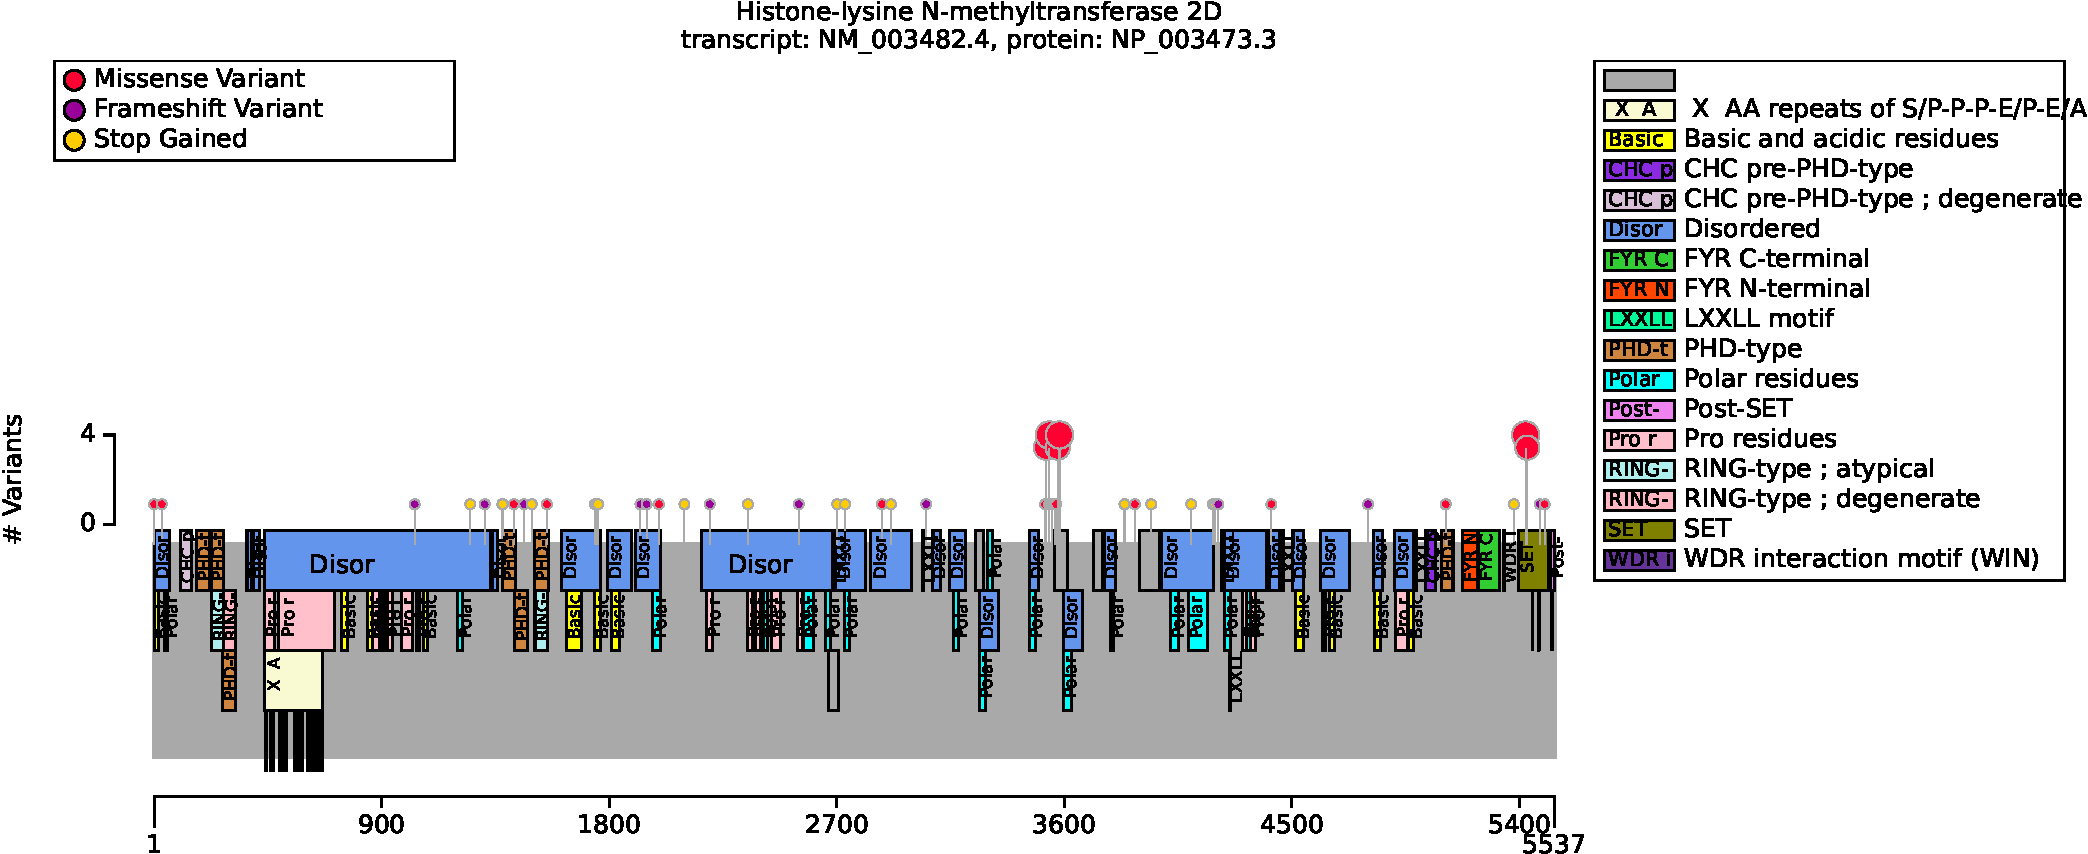
\includegraphics[width=\textwidth]{ img/KMT2D_protein_diagram.pdf} 
\captionsetup{justification=raggedright,singlelinecheck=false}
\caption{Distribution of variants in KMT2D}
\end{subfigure}

\vspace{2em}

\begin{subfigure}[b]{0.95\textwidth}
\centering
\resizebox{\textwidth}{!}{
\begin{tabular}{llllrr}
\toprule
Genotype (A) & Genotype (B) & total tests performed & significant results\\
\midrule
FEMALE & MALE & 31 & 0\\
missense & other & 31 & 0\\
n-terminal & other & 31 & 0\\
p.Glu5425Lys & other & 26 & 0\\
p.Leu3542Pro & Other variant & 5 & 0\\
\bottomrule
\end{tabular}
}
\captionsetup{justification=raggedright,singlelinecheck=false}
\caption{Fisher Exact Test performed to compare HPO annotation frequency with respect to genotypes. }
\end{subfigure}

\vspace{2em}

\caption{ The cohort comprised 65 individuals (35 females, 30 males). 5 of these individuals were reported to be deceased. A total of 151 HPO terms were used to annotate the cohort. Disease diagnosis: Kabuki Syndrome 1 (OMIM:147920). . A total of 65 unique variant alleles were found in \textit{KMT2D} (transcript: \texttt{NM\_003482.4}, protein id: \texttt{NP\_003473.3}).}
\end{figure}
